\documentclass{standalone}
\usepackage{tikz, xcolor}
\usetikzlibrary{calc, quotes, arrows}
\usepackage{tikz-dimline}

\definecolor{okinawaRed}{HTML}{C8003C}

\begin{document}
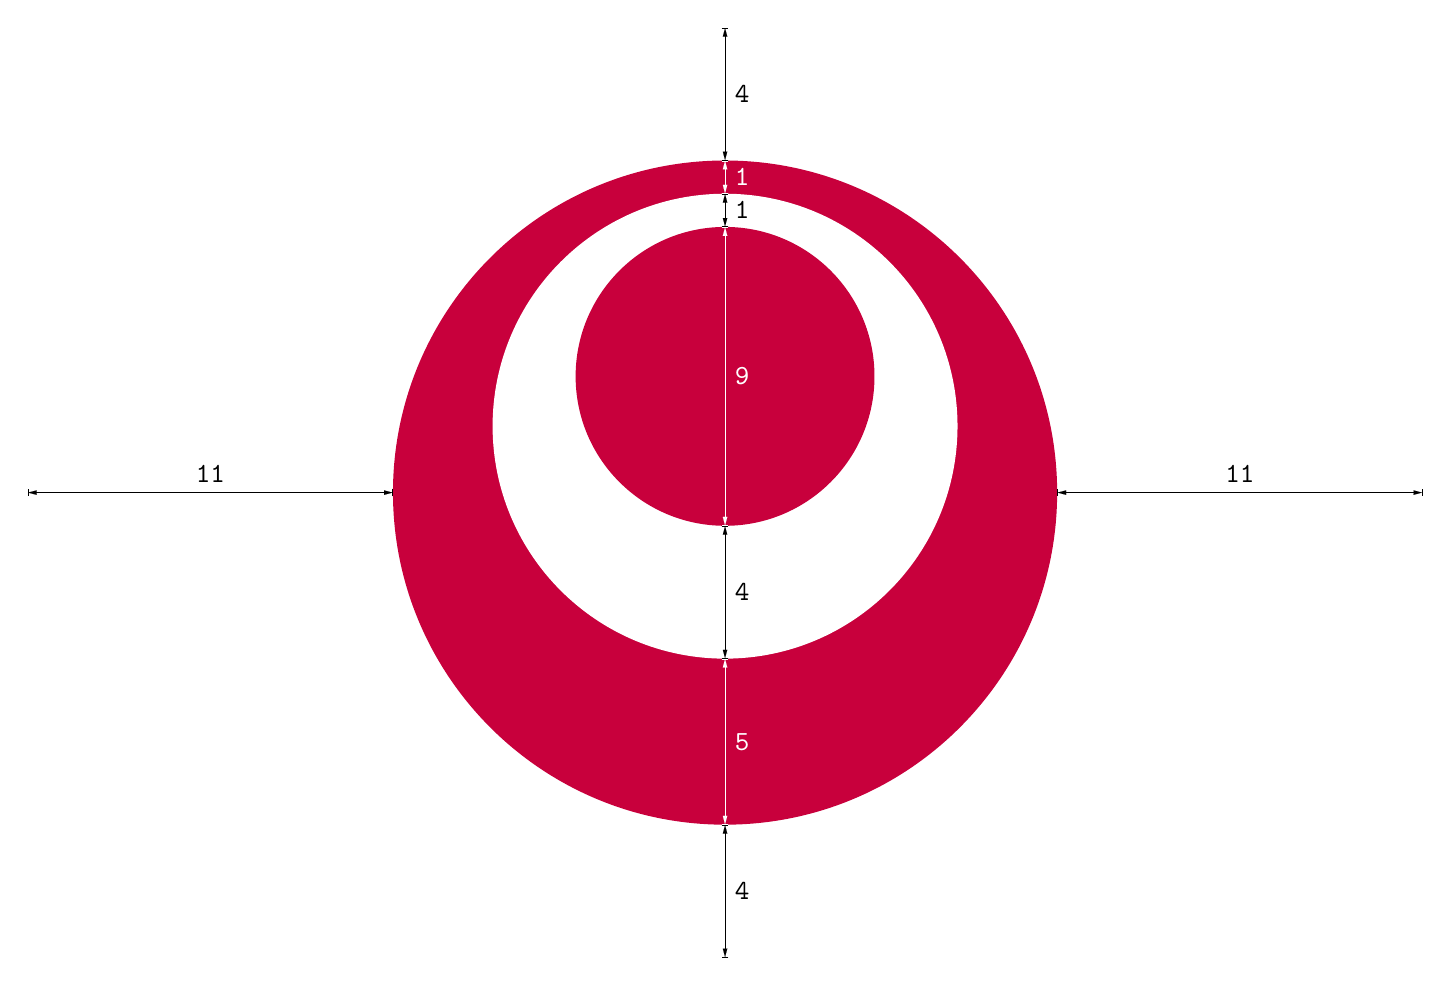
\begin{tikzpicture}[x=12pt,y=12pt]
    \fill[use as bounding box, white] (-21,-14) rectangle (21,14);
    \fill[okinawaRed] (0,0-10) arc (-90:270:20*0.5);
    \fill[white]      (0,5-10) arc (-90:270:14*0.5);
    \fill[okinawaRed] (0,9-10) arc (-90:270: 9*0.5);
    \path[
        dimline-dimline,
        every node/.style={font=\ttfamily},
    ]
    (0, 14) edge["4",black] (0, 10)
    (0, 10) edge["1",white] (0,  9)
    (0,  9) edge["1",black] (0,  8)
    (0,  8) edge["9",white] (0, -1)
    (0, -1) edge["4",black] (0, -5)
    (0, -5) edge["5",white] (0,-10)
    (0,-10) edge["4",black] (0,-14)
    (-21,0) edge["11",black] (-10,0)
    ( 10,0) edge["11",black] ( 21,0);
\end{tikzpicture}

\end{document}
